\documentclass[]{report}

\usepackage[utf8]{inputenc}
\usepackage[T1]{fontenc}
\usepackage{lmodern}
\usepackage[polish]{babel}
\usepackage{amsmath}
\usepackage{amsfonts}
\usepackage{amssymb}
\usepackage{graphicx}
\usepackage{graphics,epsfig}
\usepackage[]{animate}
\usepackage{xmpmulti}
\usepackage{media9}
\RequirePackage{xcolor}
\usepackage{blindtext} % Package to generate dummy text throughout this template 

\usepackage[sc]{mathpazo} % Use the Palatino font
\usepackage[T1]{fontenc} % Use 8-bit encoding that has 256 glyphs
\linespread{1.05} % Line spacing - Palatino needs more space between lines
\usepackage{microtype} % Slightly tweak font spacing for aesthetics
\usepackage[english]{babel} % Language hyphenation and typographical rules
\usepackage[hang, small,labelfont=bf,up,textfont=it,up]{caption} % Custom captions under/above floats in tables or figures
\usepackage{booktabs} % Horizontal rules in tables
\usepackage{lettrine} % The lettrine is the first enlarged letter at the beginning of the text
\usepackage[utf8]{inputenc}
\usepackage{enumitem} % Customized lists
\setlist[itemize]{noitemsep} % Make itemize lists more compact

\usepackage{abstract} % Allows abstract customization
\renewcommand{\abstractnamefont}{\normalfont\bfseries} % Set the "Abstract" text to bold
\renewcommand{\abstracttextfont}{\normalfont\small\itshape} % Set the abstract itself to small italic text

\usepackage{titlesec} % Allows customization of titles
\renewcommand\thesection{\Roman{section}} % Roman numerals for the sections
\renewcommand\thesubsection{\roman{subsection}} % roman numerals for subsections
\titleformat{\section}[block]{\large\scshape\centering}{\thesection.}{1em}{} % Change the look of the section titles
\titleformat{\subsection}[block]{\large}{\thesubsection.}{1em}{} % Change the look of the section titles

\usepackage{fancyhdr} % Headers and footers
\pagestyle{fancy} % All pages have headers and footers
\fancyhead{} % Blank out the default header
\fancyfoot{} % Blank out the default footer

\fancyfoot[RO,LE]{\thepage} % Custom footer text

\usepackage{titling} % Customizing the title section

\usepackage{hyperref} % For hyperlinks in the PDF

%----------------------------------------------------------------------------------------
%	TITLE SECTION


% Title Page
\title{Adsorpcja Languimira. Kinetyczne Monte Carlo (KMC)}
\author{Roksana Szwarc}


\begin{document}
\maketitle

\begin{abstract}
	 Celem projektu było zbadanie zależności pokrycia powierzchni od czasu $\theta (t)$ oraz osiąganie równowagi dla 3 przypadków:  $r_A/r_D = 2$, $r_A/r_D = 1$  oraz $r_A/r_D =1/4$. W chwili początkowej przyjęłam zerowe pokrycie powierzchni $\theta (t = 0) = 0$. Pierwszym krokiem było wykonanie symulacji z użyciem języka c++. Następnie z użyciem programu Mathematica 12.0 rozwiązałam problem metodą MFA i porównałam wyniki otrzymane dwoma metodami.
\end{abstract}
\subsection{Osiąganie równowagi w adsorpcji Languimira. Omówienie tematu}
Na przykładzie modelu gazu sieciowego przyjęłam, że wolne węzły stanowią miejsca adsorpcyjne(NA), a obsadzone węzły reprezentują zaadsorbowane cząstki(ND). Liczba węzłów N = NA+ ND. Puste węzły sieci kwadratowej (miejsca adsorpcyjne) są losowo obsadzane. Cząstki z fazy gazowej mogą być adsorbowane na powierzchni w miejscach adsorpcyjnych z rate $r_A$. Natomiast proces desorpcji (przechodzenia zaadsorbowanych cząstek do fazy gazowej) będzie zachodził z rate  $r_D$. 
\subsection{Rozwiązanie za pomocą symulacji z użyciem języka c++}
Algorytm tworzyłam bazując na wcześniej wymienionych założeniach. Jako warunki początkowe przyjęłam ilość węzłów sieci N na poziomie 10000, NA na poziomie 10000 oraz ND równe 0. Początek symulacji miał miejsce w chwili t=0. Dodatkowo pominęłam oddziaływanie między cząstkami, co sprowadziło algorytm do  uaktualniania dwóch grup: zdarzeń z grupy adsorpcji lub desorpcji. Wybrałam liczbę losową w zakresie od zera do R, gdzie R jest parametrem rozkładu Poissona. W tym przypadku łącznego rozkładu zdarzeń adsorpcji i desorpcji.  Jeśli wylosowana liczba była mniejsza od $r_A$ to zachodziła adsorpcja, w przeciwnym przypadku desorpcja. W przypadku zajścia zdarzenia aktualizowałam stan układu, a następnie dokonywałam aktualizacji czasu. Zmianę pokrycia w czasie możemy opisać następującym równaniem kinetycznym:
$\frac{d \theta}{d t}=r_{A}(1-\theta)-r_{D} \theta$.
By przedstawić tę zależność w języku c++ wprowadziłam wielkość $\theta$ opisującą pokrycie powierzchni adsorbatem, $\theta$= ND/N. Obliczałam ją dla każdego kolejnego kroku czasowego, a następnie zapisywałam wartość czasu i wartość $\theta$ do pliku tekstowego. Następnie dokonałam eksportu danych do programu Mathematica 12.0, w którym wygenerowałam wykres 1 przedstawiający zależność pokrycia powierzchni od czasu $\theta (t)$. 
\begin{figure}
	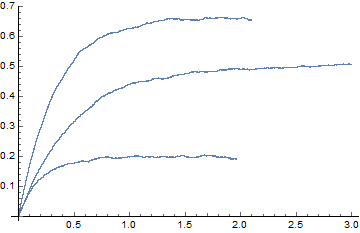
\includegraphics[width=0.8\textwidth]{Wykres1.png}
	\caption{Wykres zależności pokrycia powierzchni od czasu. Wyniki symulacji napisanej z użyciem języka c++.}
	\label{fig:W1}
\end{figure}


\subsection{Rozwiązanie MFA}
Rozwiązanie problemu metodą MFA polegało na rozwiązaniu w sposób analityczny następującego równania kinetycznego dla warunku początkowego q(t=0)=0:
$\theta(t)=\frac{r_{A}}{r_{A}+r_{D}}\left(1-e^{-\left(r_{A}+r_{D}\right) r}\right)$.
Rozwiązując powyższe równanie z użyciem programu Mathemtica 12.0 wygenerowałam wykresy zależności pokrycia powierzchni od czasu $\theta (t)$ oraz osiąganie równowagi dla 3 przypadków:  $r_A/r_D = 2$, $r_A/r_D = 1$  oraz $r_A/r_D =1/4$. Zmianę czasu ustaliłam na poziomie 3/100 w zakresie dla czasu t[0,3]. Wyniki przedstawiłam na wykresie 2. Wykresy funkcji dla 3 przypadków:  $r_A/r_D = 2$, $r_A/r_D = 1$  oraz $r_A/r_D =1/4$ oznaczone są kolejno kolorami:  różowym, błękitnym i zielonym.

\begin{figure}
	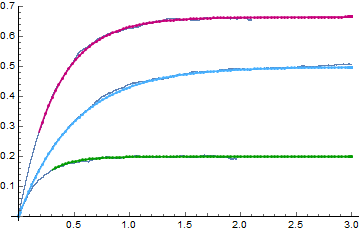
\includegraphics[width=0.8\textwidth]{Wykres2.png}
	\caption{Wykres zależności pokrycia powierzchni od czasu. Porównanie wyników symulacji w c++ oraz uzyskanych metodą MFA.}
	\label{fig:W2}
\end{figure}

\section{Wyniki}
Dane uzyskane metodą MFA są wynikiem analitycznego rozwiązania równania kinetycznego. 
W wyniku tych kalkulacji uzyskałam zależność pokrycia powierzchni od czasu $\theta (t)$. Jak widać na wykresie 2 wyniki oznaczone kolejno kolorami różowym, błękitnym i zielonym odpowiadają stosunkom rate $r_{A}/r_{D}$  równe 2, 1, 1/4. Na wykresie porównałam wyniki z wynikami uzyskanymi w wyniku symulacji w programie c++, omówionymi wyżej. 
\section{Wnioski}
Wyniki uzyskane w wyniku symulacji oraz z użyciem metody MFA są do siebie bardzo zbliżone, co widoczne jest na wykresie nr 2. Istotne są fluktuacje, które widoczne są na wykresie 1 oraz jako odchylenia od wykresów funkcji uzyskanych metodą MFA na wykresie 2. Fluktuacje mogą doprowadzić do odmiennych wyników niż tych uzyskanych w wyniku rozwiązywania w sposób analityczny ww. omówionego równania kinetycznego. Wykresy uzyskane za pomocą metody MFA charakteryzują się tym, że są gładkie. Wykresy uzyskane w wyniki przeprowadzonej symulacji z użyciem języka c++ charakteryzują się widocznymi odchyleniami od wykresów MFA - widoczne są fluktuacje. Wynika to z przedstawienia wyników jednej iteracji. Uśrednienie nastąpiłoby po wielu ewolucjach układu. 


 
\end{document}          
